%\chapter{Примеры применения интегральных уравнений в энергетике} \label{chapt1_intro}
%\chapter{Применения интегральных уравнений в энергетике} \label{chapt1_intro}
\chapter{Аналитический обзор применения методов компьютерного зрения в решении задач антропометрии} \label{chapt1_intro}

В данной главе представлен аналитический обзор алгоритмов и методов компьютерного зрения в антропометрии на основе анализа статических изображениях и видео в режиме, бликом к реальному времени. Приведены их преимущества и недостатки. Рассматривается возможности использования методов и алгоритмов компьютерного зрения для извлечения признаков.

% \section{Пример из моделирования развивающихся динамических систем} \label{sect3_2}
\todo[inline,color=cyan]{Вставить абзац связи АНТРОПОМЕТРИИ с МЗ. Иначе не понятно, что это вы тут распинаетесь по поводу МЗ. Пусть этот абзац будет пропедевтическим.}

\section{Задачи и развитие систем машинного зрения} \label{chapter1.1}

\mrk{МЗ и его краткая история}\emph{Машинное зрение}(МЗ) -- это междисциплинария область\cEA{А нормальное определение есть?}, получившая в настоящее время широкое развитие. Концепция обработки изображений и МЗ является важным разделом компьютерного зрения и основана на комбинации многих дисциплин. Прогресс в области компьютерного зрения определяется развитием математической теории\cEA{Теорией чего?}, численных методов, а также развитием вычислительных ресурсов, в частности, аппаратного обеспечения\cEA{?смартфонов?}. Долгое время теоретические исследования в области МЗ опережали вычислительные возможности ЭВМ, что затрудняло их использование для решения практических задач. В \cite{Paragios2008} условно выделен ряд этапов развития средств зрения МЗ и отмечено, что только с 1970-х годов XX века появилась возможность обрабатывать большие наборы данных. С тех пор концепции и методы МЗ привлекают все большее внимание.

\mrk{Структура МЗ.}
Системы МЗ включают\cEA{Можно добавить картинку-архитектуру} в себя следующие основные компоненты \cite{Rosenfeld2000}:
\begin{itemize}
	\item Подсистему формирования изображений, которая сама, как правило, включает разные компоненты, например, оптическую систему, осветщение и ПЗС- или КМОП-матрицу;
	\item Вычислитель;
	\item Алгоритмы анализа изображений, которые могут реализовываться программно на процессорах общего назначения, аппаратно в структуре вычислителя и даже аппаратно в рамках подсистемы формирования изображений.
\end{itemize}

\mrk{МЗ - важнейший источник информации для ИИ. Приложения.}
МЗ предоставляет важнейшую информацию для создания систем искусственного интеллекта. Такие системы могут получать информацию как из полученных  изображений так и из наборов многомерных данных различной природы \cite{Fan2013}. Сочетание машинного зрения с другими областями, такими как: информационные технологии, связь, электроника, автоматическое управление и т.д. дает нам множество применений в области науки, безопасности, военной , медицины, промышленных роботов и т.д.

\mrk{Применение МЗ -- повторение}
В последние годы проводятся научно-исследовательские работы в различных областях обработки и распознавания изображений. Машинное зрение стало самостоятельной дисциплиной \cite{Huang1991, Kevin1991}. В настоящее время методы машинного зрения реализованы во множестве устройств, применяются технологии обработки и управления, на основе изображения. Приведем краткий обзор приложений систем машинного зрения в робототехнике.

\subsection{Машинное зрение в робототехнике}

\mrk{Структура МЗ роботов и решаемые задачи.}
Система МЗ роботов является интегрированной системой, включающей одну или несколько камер \cite{Abebe2016}. В зависимости от назначения, система должна обнаруживать положение объектов в поле зрения камеры (ROI, Region of Interest). На основе этой системы, робот решает задачи определения местоположения и направления движения объектов. Для достижения высокой эффективности\cEA{Критерии эффективности? Или ж речь идет о режиме реального времени} работы необходимо обеспечивать эффективную совместную работу системы, включая аппаратные средства и программное обеспечение \cite{Zhu2004, Vayda1991}.

\mrk{Применение МЗ в промышленности.}
В современной промышленности системы компьютерного зрения роботов применяется в различных областях, таких как:
\begin{itemize}
	\item автомобильная промышленность с автоматизированными системами сборки и обработки двигателей, автомобильных кузовов;
	\item пищевая промышленность, например, система контроля автоматического закрывания пакета, закрывания контейнера  обнаружения посторонних предметов в пище при упаковке;
	\item фармацевтическая промышленность: контроль упаковки и партии, обнаружение дефектов;
	\item военно-силовые структуры: обнаружение целей беспилотными летательными аппаратами, анализ багажа, анализ поведения групп людей в общественных местах.
	\item обеспечение безопасности, предупреждение преступности в том числе \cEA{Распознавание чего делается? -- много неопределенности}на основе антропометрических признаков;
	\item индустрии развлечений и спорта: системы автоматического управления камерой слежения за объектами в футбольном матче, гонках и т.д.
\end{itemize}

\mrk{Классы задач МЗ в робототехнике.}
Таким образом, современная робототехника требует решения многих сложных задач МЗ, в том числе следующих:
\begin{itemize}
	\item ориентация во пространстве и определение расстояний до объектов;
	\item распознавание и классификации различных объектов, интерпретации сцен, навигация;
	\item обнаружение людей, распознавание их лиц и анализ эмоций;
	\item восстановление изображений и подавление шумов, повышение разрешнения изображений, в том числе получение изображений со сверхразрешением.
\end{itemize}

\subsection{Машинное обучение и информационный поиск}

\todo[inline]{Связь МЗ и машинного обучения}

\mrk{Машинное обучение и интернет-проекты}
На сегодняшний день машинное обучение используется в бесчисленном множестве интернет-проектов. У многих известных IT-компаний (к примеру, Яндекс, Google, Facebook, Microsoft) на нём базируются многие ключевые технологии \cite{Cormier2016}.

\mrk{Поиск, сравнение и классификация изображений в Интернет}
Задачи поиска изображений по содержанию также разнообразны. Они включают в себя следующие шаги \cite{Meer2000}. Сравнение содержимого изображения для обнаружения и распознавания на изображениях объектов классов\cEA{Не слищком абстрактно?} разной степени общности. Такие алгоритмы очень полезны для создания приложений, таких как: классификация данных (изображения, видео и т.д.), поиск товаров на основе изображений для интернет-магазинов, для извлечения изображений в геоинформационных системах, для систем биометрической идентификации, для специализированного поиска изображений в социальных сетях (например, для поиска лиц людей, привлекательных для пользователя) \cite{Findface} и т.д., вплоть до поиска изображений в интернете.

\mrk{МЗ-задачи решаются методами машинного обучения. -- хороший кандидат на первый абзац раздела.}
Методами машинного обучения при разработке систем компьютерного зрения решаются проблемы распознавания объектов. Разработка алгоритмов классификации является одной из важнейших областей машинного обучения \cite{Murino2000}. Методы глубокого обучения (deep learning) требуют огромных вычислительных ресурсов, и даже для обучения распознаванию ограниченного класса объектов могут требоваться несколько дней работы на вычислительном кластере. При этом в будущем могут быть разработаны еще более мощные, но требующие еще больших вычислительных ресурсов методы.  Отметим, что использование специфики решаемой задачи позволяет существенно сократить вычислительную сложность, однако требует более глубокого понимания сути решаемой задачи.

\todo[inline,color=cyan]{Ну и какая СОДЕРЖАТЕЛЬНО ПРЕДСТАВЛЕННАЯ связь М-обучения с МЗ и приложениями на производстве и робототехнике, кроме специфики задачи???}

\subsection{Мобильные приложения машинного зрения}

\mrk{МЗ на моб.устройствах. Фичи мобил}
Задачи компьютерного зрения все шире используются в приложениях для персональных мобильных устройств, таких как смартфоны, планшеты и прочее. В частности, число смартфонов неуклонно растет и уже практически превысило по численности население земли \cite{Battiato2012}. Часть задач по обработке изображений для мобильных устройств с камерами совпадает с задачами для цифровых фотоаппаратов. Основное отличие заключается в качестве объективов и в условиях съемки. В спектре аппаратного обеспечения, доступного для решения задач отметим модули с доступом к интернет, наличия интернета, GPS и конечно мощного процессора и большой памяти. Именно с этим связано появление такого термина, как <<smart phone>> \cite{Hannuksela2007}.

\mrk{???? + МЗ+Дополненная реальность....???}
В этой связи решение, казалось бы, идентичных задач для разных устройств может различаться, что делает эти решения высоко востребованными на рынке. Приложения для смартфонов выходят на рынок, наблюдается огромный интерес к компьютерному зрению и приложений дополненной реальности в мобильных устройствах \cite{Shubina2010}.

\mrk{Примеры задач МЗ на мобилах}
В настоящее время существует много приложений, использующих обработку изображений, для мобильных устройств. Например, программа автоматической коррекции лицевых дефектов (таких, как морщины, угри, веснушки) в соответствии с заданным стилем (натуральный, классический, контраст и т.д.). Это такие приложения, как camera360, Perfect Selfie. Приложения по обработке изображений на видео позволяют пользователям создавать тематические видео из фотографий, анимации и т.д. -- MiniMovie, Imovie-editing и Маскарад, которые преобразует видео в стиль картин художника Ван Гога и мультипликации.

\mrk{Задачи ориентации, распознавание кепоинтов. ДОПИСАТЬ ПРИМЕРЫ.}
Более сложные задачи, связанные с сопоставлением (отождествлением сопряженных точек) на изображениях, оценкой трехмерной структуры сцены, определением изменения ориентации камеры, распознавание объектов, а также анализа лиц людей, также находят свои приложения в\ldots{}\cEA{Привезти примеры.}. Повышение качества решения перечисленных задач требует совершенствования и разработки нового математического и программного обеспечения, и адаптации его к вычислительным возможностям мобильных устройств, а также к их периферии.

\mrk{Резюме - МЗ на мобилах - это круто.}
Перечисленные примеры и задачи показывают, что класс приложений МЗ на мобильных устройствах крайне широк и любое продвижение в развитии и исследовании методов обработки изображений является актуальным.
\todo[inline,color=cyan]{Какая связь СОДЕРЖАНИЯ РАЗДЕЛА с АТРОПОМЕТРИЕЙ?}

%%% Local Variables:
%%% mode: latex
%%% TeX-master: "../dissertation"
%%% End:

%-------------------------
\section{Анализ алгоритмов и методов компьютерного зрения для извлечения признаков в антропометрии}

Использование современных методов компьютерного зрения позволяет разрабатывать новые подходы к автоматизации различных адач антропометрии. Компьютерное зрение предоставяляет большой арсенал методов для решения задач антропометрии. Условно такие задачи можно разбить на следующие этапы: калибровка, регистрация изображения (или видео), обнаружение объекта (человека), сегментация и выделение признаков (антропометрических измерений). Дополнительно может понадобиться классификация признаков и  построение 3D модели человека (это будет рассмотрено ниже) \cite{Rebak2016}.

\subsection{Антропометрические признаки}

Изображение представлено матрицей пикселей. Изображение содержит различные функции, это зависит от содержания каждого изображения. Исходя из нашей цели необходимо реализовать алгоритмы извлечения признаков, чтобы достичь наилучшей точности, устойчивости и скорости антропометрии.

Итак, первая задача состоит в использовании и преобразовании изображения в вектор признаков. По сути это представление информации в более сжатом виде в зависимости от решаемой задачи. 

Признак (feature)  $f$  объекта $a$ – отображение $f:A\rightarrow D_f$  где $D_f$ – множество допустимых значений признака \cite{Mecte2002}.  Если имеется набор признаков $f_1,…,f_n$, то вектор $x= \left(f_1\left(a\right), ..., f_n\left(a\right)\right)$ называется признаковым описанием объекта $a\in A$. Признаковые описания с определенными ограничениями допустимо отождествлять с самими объектами. При этом множество $A=\left(D_{f_1}\times ... \times D_{f_n}\right)$ называют признаковым пространством (feature space, пространство признаков). Задаче извлечения признаков объектов, как правило, предшедствуют этапы обнаружения и сегментации объектов. 
Антропометрические признаки выражены в форме и размерах частей человеческого тела (рис. \ref{img1}).
\begin{figure}[htb]
\centering
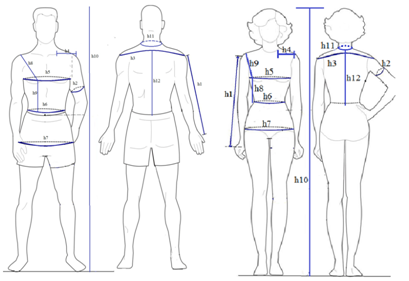
\includegraphics [scale=0.8] {images/h1.png}
\begin{center}
%\captionsetup{justification=justified, labelsep=period}
\caption{Описание антропометрических признаков.} \label{img1}
\end{center}
\end{figure}

Признаки формы. Форма объекта или области является важной характеристикой при обнаружении и классификации изображений в распознавании образов \cite{Jones2002}, \cite{Dubinskiy2003}. Основная цель анализа формы состоит в измерении геометрических свойств объекта, используемых в классификации, сравнения и распознавания объектов \cite{Kpalma2006}. Так, в области антропометрии, антрометрической характеристикой является размер частей человеческого тела. Он состоит из следующих величин \cite{urlclothes2015}: рост, длина рук, длина ног, окружность талии, окружность грудной клетки, окружность бедер и т.д. Современные антропометрические измерения могут служить основой для 3D моделей человеческого тела\cite{Toldo2009}, \cite{Ponce1989}, \cite{Zhang2001}.

Использование цвета кожи в ввиде признаков. Цвет является отличительной особенностью и используется для алгоритма обнаружения кожи \cite{Fink2006}. Каждый пиксель (информация о цвете) может быть представлен в виде трехмерной точки в определенном цветовом пространстве \cite{Albio2001}, \cite{Shin2002}. Общие цветовые пространства: RGB, Munsell, CIE, HSV \cite{Jones2002}.

\subsection{Извлечение антропометрических признаков}

Приведем краткий обзор исследований, посвященных применению методов компьютерного зрения к решению задач антропометрии, анализу положений человека и создания 3D-моделей. Для статических изображений было сделано несколько научно-исследовательских работ для того, чтобы обнаружить человеческое тело, используя описание фона и модели человеческого тела \cite{Mori2002}. В \cite{Belongie2002} представлен алгоритм сегментации частей тела на основе силуэта. Данный подход делит тело на основе использования контура каждой области на теле человека. Авторы отмечают, что их алгоритм выполняется плохо, когда части тела, особенно руки, держатся близко к телу. Авторы \cite{Mittal2003} продемонстрировали, что использование искусственно сгенерированных данных обучения помогает произвести сегментацию человеческого контура, взятого из шумных изображений реального силуэта. Авторы утверждают, что такая сегментация должна хорошо работать, несмотря на шум в исходных данных.

Извлечение антропометрических признаков выбирается на основе 2D-изображений. Оно предоставляет данные для многих приложений. Например: бесконтактное измерение размеров человеческого тела \cite{Lin2008}, построение 3D моделей \cite{Lin2010}, \cite{Lin2012}, распознавание человеческих действий \cite{Ikizler2008}. 
В работе \cite{Gopal} предложена методика сочетания наборов данных (PCD) для синтеза антропометрических баз данных на основе легкодоступной информации о значениях измерения различных областей человеческого тела. Авторы собрали такие данные для улучшения анализа перемены населения. Метод состоит из трех этапов: сбор описательной статистики о антропометрии, подгонка антропометрических моделей к этой информации, а также формирование антропометрической модели для генерации необходимых данных. Применение этой процедуры продемонстрировано на двух базах данных: военных США в конце 1980-х и японской молодежи в начале 1990-х годов. Методика является простой, легко применимой и точной. В данной статье \cite{Adams} представлен количественный анализ качества данных, собранных в ходе опроса населения волонтерами.  В результате обследования населения были получены данные артериального давления и антропометрии. На протяжении всего исследования собраны антропометрические данные и кровяное давление, которые были в пределах допуска для ошибок, установленных в начале исследования. В статье \cite{Jiang2012} предлагается подход для автоматического обнаружения ключевых точек контура человеческого тела. Этот метод применяется к изображениям, в которых имеется две раличные  позы (стоя в профиль и анфас). Реализуется он следующим образом: во-первых, используется эффективный подход к обнаружению формы тела - метод на основе обнаружения края \cite{Canny1986} и 8-связного цепного кода Фримэна \cite{Freeman1961}. Затем определяются взаимосвязанные регионы. Ряд характерных точек извлекается на основании указанных правил путем измерения разности между областями сегментов. В общей сложности 101 характерная точка с четкими геометрическими свойствами извлекаются автоматически, в том числе 27 точек, соответствующих определений ориентиров об измерениях швейной индустрии. Наконец, предлагаемый подход был протестирован на человеческих субъектах, и целых 101 характерных точек с конкретными геометрическими характеристиками были правильно извлечены, что свидетельствует об эффективной и надежной работы (рис. \ref{img2}).

\begin{figure}[ht!]
\centering
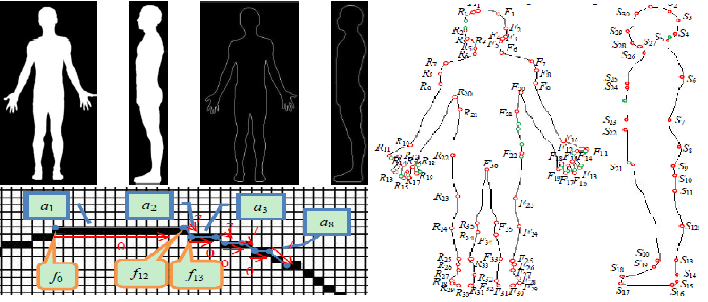
\includegraphics [scale=0.8] {images/h2.png}
\begin{center}
%\captionsetup{justification=justified, labelsep=period}
\caption{Маркировка контура в методе извлечения антропометрических признаков на основе ключевых точек \cite{Lin2008}.} \label{img2}
\end{center}
\end{figure}

В работе \cite{Nevatia2009} предложен метод обнаружения объектов в случае их частичной видимости в поле зрения. Метод апробирован на видеопотоке уличных сцен. Основной вклад этого метода включает:

\begin{itemize}
	\item Проектирование иерархии для процесса обучения путем деления признаков;
	\item Метод сегментации объектов на основе  классификатора AdaBoost.
\end{itemize}

Ioffe и Forsyth \cite{Ioffe2001} предложили методы автоматизации антропометрии, основанные на обнаружении частей тела человека. Их система подразумевает, что человек одет в специальную одежду. Определения сегментов для определения ключевых точек тела, необходимых для правильного измерения длины сегментов тела встречаются в \cite{Leva1996}. 

\begin{figure}[ht!]
\centering
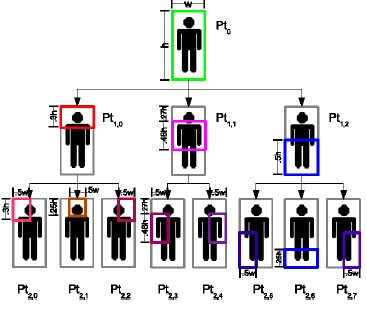
\includegraphics [scale=0.8] {images/h3.png}
\begin{center}
%\captionsetup{justification=justified, labelsep=period}
\caption{Описание системы обнаружения объекта на основе обнаружения каждой его части \cite{Nevatia2009}.} \label{img3}
\end{center}
\end{figure}

На (рис. \ref{img3}) представлена часть обнаружения тела человека на основе каскадных признаков и метода классификации на основе boosting. Программа включает в себя 3 этапа: 1) обнаружение человека, 2) обнаружение верхней части тела, средней и нижней частей тела, 3) соотнесение различных частей человеческого тела. Используется следующая классификация : верхняя часть тела (голова, правая, левая часть лица), средняя часть тела (правая рука, левая рука), нижняя часть тела (правая нога, левая нога, ноги). 

Кроме того, улучшен метод, использующий математические модели формы (3D-сканирование) для извлечения антропометрических признаков. В \cite{Baek2012} авторы предложили построение модели, которая состоит из трех основных этапов: построение базы данных, статистического анализа и генерации модели. База данных была собрана из 250 3D-сканов всего тела. Данные обрабатываются, чтобы сделать ввод данных для статистического анализа (рис. \ref{img4}). Используется соотношение частей человеческого тела для построения 3D модели. Система определяет местоположение и форму каждой части тела и вычисляет её размер. По сравнению с другими параметрическими методами моделирования человека \cite{Siebert2000}, \cite{Seo2001}, их метод вносит свой вклад путем введения нового способа соотношения формы и размеров тела путем создания усовершенствованной техники оптимизации параметров для генерации математической модели тела человека.

\begin{figure}[ht!]
\centering
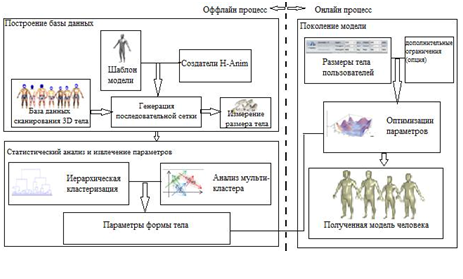
\includegraphics [scale=0.8] {images/h4.png}
\begin{center}
%\captionsetup{justification=justified, labelsep=period}
\caption{Описание метода извлечения антропометрических признаков на основе сканирования тела \cite{Baek2012}} \label{img4}
\end{center}
\end{figure}

Авторы в работе \cite{Blanz1999} также предложили метод математического моделирования формы человеческого тела. Система собирает данные путем 3D сканирования человеческого лица. Система анализирует полученные данные на основе основного метода главных компонент - PCA. Используя эту специальную базу данных, можно проанализировать и извлечь доминирующие переменные, определяющие форму лица. Используя идеи статьи \cite{Blanz1999}, Allen \cite{Allen2003} установил набор 3D данных сканирования тела. Был разработан новый способ генерации последовательной структуры сетки путем аппроксимации на основе шаблонов. В \cite{Seo2003}, \cite{Seo2004} авторы предложили использовать нейросетвой подход в этой задаче. Этот подход показал высокую эффективность для соотнесения размера фактического человеческого тела с размером тела базы данных. Критическую роль в этом подходе играет процесс обучения. Была обнаружена зависимость между формой и размерами человеческого тела. На основе этих отношений, система синтезирует новую модель с размером тела путем сопоставления формы в базе данных. Стандартные сканеры обычно используют бинарные модели, состоящие из черных и белых полос.  Этот подход подвержен ошибкам из-за зависит от разрешения и шума \cite{Rocchini2001}. Кроме того, это также зависит от расстояния между объектом и устройством. Это влияет на результаты восстановления изображения на основе данных, которые получены со сканера. Система работает эффективно даже в условиях низкой освещенности. Другой подход, основанный на компьютерном зрении изложен в работе \cite{Taeyoung2015}. Система состоит из четырех основных этапов: обработки изображений на основе вычитания фона и распознавания маркера, обработки инфракрасных изображений для надежного обнаружения маркера, для проектирования ортопедических стелек с учетом индивидуальных особенностей (рис. \ref{img5}).

\begin{figure}[ht!]
\centering
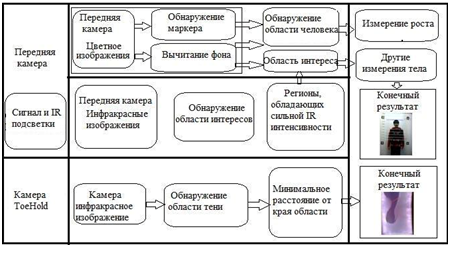
\includegraphics [scale=0.8] {images/h5.png}
\begin{center}
%\captionsetup{justification=justified, labelsep=period}
\caption{Описание системы извлечения антропометрических признаков в остеопатии\cite{Taeyoung2015}.} \label{img5}
\end{center}
\end{figure}

Эта тема получила развитие в работах \cite{McCulloch1988} и \cite{Lee2000}.

%-------------------------
\section{Анализ методов машинного обучения для классификации признаков}

В настоящее время существует множество методов и алгоритмов компьютерного зрения, предложеных и развитых для классификации данных.

Особенности систем машинного зрения позволяют вырабатывать требования для разработки методов и алгоритмов классификации. Кроме того, тип данных является решающим фактором адекватности и точности классификации \cite{segi1998}, \cite{sophi2000}. Было много исследований в которых успешно применяются алгоритмы и методы компьютерного зрения для классификации данных, таких как распознавание жестов \cite{Phan2013}, распознавание лиц \cite{Phakhi2013, Goldstein1991}, идентификация деятельности человека \cite{Kang2006, Saaidi2008}. Адаптивные методы распознавания объектов и классификации основаны на автоматической подстройке к свойствам обрабатываемых данных, что позволяет разработать распознающую систему с приемлемыми характеристиками \cite{anwef2011}. Ко второй категории относятся методы, характеризующиеся сокращением размерности данных \cite{Belhumeur1997}, \cite{Hallinan1999}. Ниже изложим наиболее популярные методы классификации.

\subsection{Алгоритм AdaBoost}

Алгоритм AdaBoost был разработан Йоавом Фройндом (Yoav Freund) и Робертом Шапиром (Robert Schapire) в 1996 году \cite{Freund1997}, \cite{Freund1996}. Этот алгоритм <<адаптивность и усиление>> используется для создания классификатора. Как известно, классификатор на входе принимает набор данных для обучения и пытается предсказать или классифицировать новые образцы данных, которые относятся к определенному классу \cite{Sochman2004} (рис. \ref{img6}). Алгоритм AdaBoost построен на основе алгоритмов обучения (например, деревья решений) и объединения их. Цель состоит в том, чтобы создать один сильный классификатор на основе нескольких слабых классификаторов. Алгоритм AdaBoost успешен в поиске личной информации на статических изображениях \cite{Su2005}. Сайты постоянно поддерживают поиск информации на основе изображений используя AdaBoost.

Система поиска лица на основе алгоритма <<Viola-Jones>> \cite{Viola2001}, \cite{Violaj2001} также использует AdaBoost. Эти системы работают с высокой точностью, например в цифровых фотокамерах и смартфонах. Вейвлет Хаара \cite{Viola2004} являются одним из простых признаков, которые обычно используется на практике. Но размер такого вектора-признака довольно большой (162,336). Таким образом, нужно применять метод главных компонентов (англ. principal component analysis, PCA) \cite{Masoud2005} для увеличения или уменьшения размера и выбора новых функций. После этого полученные данные классифицируются алгоритмом AdaBoost.


\begin{figure}[ht!]
\centering
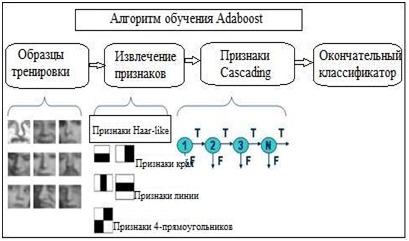
\includegraphics [scale=0.8] {images/h6.png}
\begin{center}
%\captionsetup{justification=justified, labelsep=period}
\caption{Описание алгоритма AdaBoost \cite{Sochman2004}.} \label{img6}
\end{center}
\end{figure}

Этот алгоритм прост и удобен а также, имеет очень высокую скорость обучения.  Алгоритм AdaBoost гибкий и универсальный, может быть объединен с любым алгоритмом машинного обучения, и может работать с большим количеством различных данных.

\subsection{Искусственные нейронные сети}

Нейронная сеть была успешно использована для решения задач классификации объекта \cite{Hinton2012}. С точки зрения машинного обучения, искусственные нейронные сети (ИНС) являются вычислительными моделями, которые способны решать задачи распознавания образов \cite{Sergios2006}, \cite{Dunne2007}. Нейронную сетевую архитектуру можно разделить на две основные группы: сети прямой связи \cite{Colin2000} и обратного распространения сети \cite{Kamruzzaman2006}. При решении задачи классификации возраста и пола человека применяется большое количество нейронных сетей различных архитектур \cite{Rowley1998}, в частности: вероятностные нейронные сети (probabilistic decision-based neural networks) \cite{Lin1997}, многослойные персептроны \cite{Juell1996} и т.д. Нейронные сеть - ИНС являются одним из приоритетных направлений исследований в области машинного обучения.

Действительно, искуственные нейронные сети способны решить различные проблемы: классификация образов, аппроксимации функций, оптимизация и квантование вектора пространства данных, в то время как традиционные методы не могут эффективно решить вышеуказанные проблемы.

\subsection{Метод опорных векторов}

Метод опорных векторов (Support Vector Machines, МОВ)  используется для решения задач классификации и регрессионного анализа. Этот метод был предложен В. Вапником и А. Червоненкисом в 1995 году \cite{Vapnik1995}. Особые свойства МОВ – это непрерывное уменьшение эмпирической ошибки классификации. Использование МОВ и мешка признаков (Bag-of-Features) оказалось эффективным в задачах обнаружения и распознавания жестов на видеопоследовательности \cite{Nasser2011, Dardas2010}, а также при решении других задач \cite{Jiang2007, Lazebnik2006}. Метод опорных векторов (МОВ) позволил классифицировать нормальные и ненормальные поведения человека \cite{Yogameena2010}. В работе \cite{Nguyen2015} авторы представили предлагаемый подход к классификации пола и размера одежды с помощью метода опорных векторов. Алгоритм работал с антропометрическими данными для классификации по двум классам: мужчины / женщины.

Метод опорных векторов, как и методы на основе деревьев решений даёт высокую точность для наборов данных с непрерывными типами данных (непрерывное значение). Они являются двумя методами, которые обычно используются для классификации данных. Тем не менее, не существует универсального метода классификации. Результат всегда зависит от цели системы и типов данных. Кроме того, выбор ядра и других параметров является  слабостю МОВ.

\subsection{Алгоритм случайного леса (Random Forest)}

Random Forest (случайный лес) \cite{Breiman2002, Breiman2001} является развитием семейства алгоритмов, разработанных Лео Брейман в университете Калифорнии, Беркли. На самом деле, Random Forest использует методы, называемые мешки (bagging). Эта методика позволяет выбрать подмножество атрибутов в каждом узле дерева классификатора, чтобы разделить его на следующий уровень. Таким образом, Random Forest имеет возможность разделить очень большое пространство поиска на меньшие пространства поиска. Таким образом, алгоритм может выполнять сортировки быстро и легко.

В случайном лесе, разработка набора деревьев значительно улучшила точность классификации, каждое дерево в наборе будет <<голосовать>> за самый популярный класс. Для развития наборов деревьев, как обычно, создаются случайные векторы. Такие векторы будут регулировать развитие каждого дерева в вышеупомянутом наборе. Для дерева $K$ в наборе, случайный вектор $\theta_k$  генерируется, независимый с генерированными векторами ранее $\theta_1, \theta_2, ..., \theta_{k-1}$, но распределение таких векторов одинаково. 

Дерево было разработано на основе обучающего множества и вектора $\theta_k$. Получается результат: подкласс $h\left(x, \theta_k \right)$ где $х$ - входной вектор. После создания большого количества деревьев, проводится голосование <<голосовать>> за самый популярный класс.

Случайный лес определяется следующим образом \cite{Biggio2011}: подкласс случайного леса, состоящий из наборов слоистой структуры дерева $\left\{h\left(x,\theta_k\right), k=1, ...,n\right\}$ где $\left\{\theta_k\right\}$- независимые векторы, также случайным образом распределенные, и каждое дерево даёт один голос для наиболее популярного класса в входном векторе $х$.

Основная идея алгоритма случайного леса:

\begin{itemize}
	\item В каждом подразделении деревьев, случайный набор m атрибутов взят из m таких атрибутов, которые участвуют в распределении деревьев;
	\item -	Первый шаг в оценке важности переменной в тренировочном наборе – тренировка случайного леса в этом наборе. Во время процесса построения модели для каждого элемента тренировочного набора считаются так называемой <<out-of-bag>> ошибкой. Затем для каждой сущности такая ошибка усредняется по всему случайному лесу.
\end{itemize}

По алгоритмам Random Forest (случайного леса) отметили, что случайный лес является хорошим методом классификации, потому что: 1) в методе Random Forest, ошибки были сведены к минимуму в результате случайного леса, синтезированию через обучения (learner), 2) случайный выбор на каждом этапе в Random Forest снизит корреляцию между учащимися в синтезе результатов. Кроме того, мы также обнаружили, что общая ошибка из слоистых лесных деревьев зависит от их индивидуальных ошибок в лесных деревьях, а также корреляции между деревьями.
%-------------------------
\section{Приложение компьютерного зрения в антропометрии}

Применение методов компьютерного зрения в антропометрии должны соответствовать следующим требованиям: быстрая скорость обработки, высокая точность, возможность создать базу данных для создания приложений на практике. Для приложений безопасности, например, используется программное обеспечение распознавания объектов на основе антропометрических признаков лиц \cite{Graham1997}, 3D моделирование \cite{Zouhour2006} для областях тестильной промышленности, здоровья. Сканеры тела все чаще используются для оценки состояния здоровья и антропометрии, напримеры Caesar project \cite{Robinette2006}, SizeUK \cite{Uk2013} and SizeUSA \cite{Usa2013}. В будущем такие системы будет развиваться для решения различных задач антропометрии.

BreuckmannBodySCAN \cite{Hexagon2016} - это система для проведения антропометрических измерений. По сравнению с ручным измерением, антропометрическое измерение демонстрирует незначительную погрешность. Однако это показывает, что автоматические антропометрические измерения, сравнимо лучше традиционного метода - вручную. Для проверки ошибок авторы используют систему на основе так называемого соотношения значительного/границы (significant/borderline). Если коэффициент > 0.9, то результат измерения является приемлемым. Преимущество этой системы состоит в том, что она не зависит от движения объекта или отсутствия движения объекта, не подверженных внешним факторам, таких как шум и т.д.

3DscannerData \cite{Sobota2009} является приложением, в котором система компьютерного зрения используется в области медицины. Система анализирует форму человеческого тела. Система позволяет проводить ряд антропометрических измерений на основе данных со сканера человеческого тела. Система позволяет анализировать и прогнозировать жир в организме человека. Системы, основанные на размере тела, по сравнению со стандартным размером, чтобы выяснить разницу. Недостатком этой системы является то, что нельзя определить точное местоположение ключевых точке на теле человека для проведения антропометрических измерений. Для повышения точности системы, авторы улучшили алгоритм обнаружения позиций учета каждой части тела. Преимущества вычислительной системы заключается в быстрой работе и не нуждается во вмешательстве  пользователя.

Некоторые интеллектуальные системы на основе компьютерного зрения были применены в текстильной промышленности. Среди них, уже существующих систем были использованы непосредственно для изготовления одежды на заказ. Поэтому, в рамках диссертации предлагается система, которая, например, может помочь портному (или сотруднику фитнес-центра) измерить размеры тела клиента автоматически. Эта система использует способ и систему, основанную на  компьютерном зрении, обеспечивая комфорт и конфиденциальность для клиентов и в целях экономии средств и удобств для заказчика такого антропометрического измерения. С помощью экспериментов, система доказала, что имеет возможность измерить размеры частей человеческого тела быстро и качественно, даже при наличии шума в исходных данных. Таким образом, система автоматического измерения человеческого тела на основе компьютерного зрения представяляет интерес в различных областях, включая швейную промышленность.

Кроме того, эта система может применяться в области фитнеса. Система помогает пользователям часто проводить антропометрическое измерение, проверкять индекс ожирения, выдавая в результате. Таким образом, работы состоит в том, чтобы на основе методов компьютерного зрения создать приложение для смартфонов для решения задач антропометрии.
%-------------------------
\section{Цель и задачи исследования}

Система компьютерного зрения в антропометрии для смартфонов включает следующие три основных этапа:
\begin{itemize}
	\item Первый этап: извлечение антропометрических признаков и создание векторов антропометрических признаков;
	\item Второй этап: классификация данных антропометрических признаков на основе данных из векторов признаков;
	\item Третий этап: Создание приложений для смартфонов на базе результатов классификации.
\end{itemize}

В данной работе осуществляется разработка алгоритмов, методов компьютерного зрения для извлечения признаков и классификации данных в статических изображениях и видео в режиме реального времени. Она актуальна из-за необходимости создания систем компьютерного зрения, которые имеют лучшую эффективность, высокую скорость обработки данных для смартфонов. Система должна соответствовать условиям работы в среде шумов и в реальном времени. Развитие этого направления может быть использовано для создания интеллектуальных приложений в областях моды, красоты, фитнеса, анализа биомедицинских изображений.

Целью диссертации является разработка алгоритмов, методов компьютерного зрения в извлечении признаков и классификации антропометрических данных для построения зрительной системы для смартфонов. Эта система используется в условиях шумов и обработки данных статических изображений и видеокадров в реальном времени.

Для достижения этих целей необходимо решить следующие задачи:

\begin{itemize}
	\item Выполнять анализ подходов с использованием алгоритмов, методов компьютерного зрения для извлечения антропометрических признаков с изображений и видеопоследовательностей и предложить наиболее подходящий подход для решения данной задачи;
	\item Исследование и применение методов калибровки для повышения точности сегментации и местонахождения, измерять размеры частей человеческого тела на изображениях и видеопоследовательностях;
	\item Разработка и реализация алгоритмов, программы извлечения и классификации антропометрических данных на основе алгоритмов, методов предложенного компьютерного зрения;
	\item Оценка и редактирование точности результата системы компьютерного зрения в антропометрии;
	\item Разработка приложений компьютерного зрения в антропологии для пошива промышленности и здоровья, фитнеса. Система работает со статическими изображениями и видео в режиме реального времени;
	\item Сравнение результатов зрительной системы в антропометрии с полученными результатами других авторов.
\end{itemize}
%-------------------------
\section{Основные результаты и выводы по главе 1}

\begin{enumerate}
	\item В этой главе анализируются алгоритмический подход, методы компьютерного зрения в извлечении антропометрических признаков со статических изображений и видеопоследовательностей:
	
	\begin{itemize}
		\item Построение признаков ключевых точек из 2D-изображений, видеокадров;
		\item Использование 3D-сканирования моделей и сопоставление точек человеческого тела в построенных моделях.
	\end{itemize}
	
	\item В данной главе анализируется алгоритмический подход, методы компьютерного зрения в классификации антропометрических данных признаков в изображениях и видеопоследовательностях. Включая:
	
	\begin{itemize}
		\item Алгоритм Adaboost;
		\item Нейронные сети;
		\item Опорных векторов (SVM).
	\end{itemize}
\item Также здесь рассматриваются возможности использования алгоритмов ICP и разреза графов (Graph-сuts) для извлечения антропометрических признаков и алгоритм случайного леса для классификации антропометрических данных в изображениях и видеопоследовательностях.
\item На основе проведенного анализа принято решение о адекватности и точности использования комбинированных алгоритмов ICP, разреза графов (Graph-cuts) для извлечения антропометрических признаков с использованием метода случайного леса (Random Forest) для классификации антропометрических данных в статических изображениях, видео в присутствии шума и в режиме реального времени. Такой подход позволяет построить систему компьютерного зрения в антропометрии с высокой точностью и скоростью обработки.
\end{enumerate}

%-------------------------

%%% Local Variables:
%%% mode: latex
%%% TeX-master: "../dissertation"
%%% End:
